\chapter{A biodiversidade em todas as escalas}\label{ch:g10:biodiversity-scales}

Estenda um quadrado de barbante de um metro de lado sobre um gramado e
conte o que cresce dentro dele: grama, claro, mas também trevo,
margaridas, um dente-de-leão, tanchagem, musgo e, se você olhar com uma
lupa, uma dúzia de insetos e um caracol. Passe o quadrado para o
asfalto do estacionamento: nada, ou uma erva daninha numa rachadura.
Passe-o para um prado antigo que nunca foi arado: quarenta \omterm{def:g10:biodiversity-scales:species}{espécies} de
plantas, e insetos além da conta. A palavra para o que o quadrado mede
é \emph{\omterm{def:g10:biodiversity-scales:biodiversity}{biodiversidade}}, e este capítulo trata de como medi-la, em que
escalas ela existe, e por que ela não é fixa nem garantida.

\section{Três escalas de diversidade}

\begin{definition}[Biodiversidade]\label{def:g10:biodiversity-scales:biodiversity}
A \emph{biodiversidade}\index{biodiversidade} é a diversidade dos seres
vivos, considerada em três escalas:
\begin{itemize}
  \item a diversidade dos \emph{ecossistemas}\index{ecossistema} ---
        das comunidades vivas e dos ambientes que elas ocupam (uma
        lagoa, uma floresta de faias, um recife de corais, um prado),
        cada um com o conjunto próprio de \omterm{def:g10:biodiversity-scales:species}{espécies};
  \item a diversidade das \omterm{def:g10:biodiversity-scales:species}{espécies} dentro de um
        ecossistema ou na Terra --- o número de \omterm{def:g10:biodiversity-scales:species}{espécies} e a abundância
        relativa delas;
  \item a \emph{diversidade genética}\index{diversidade genética}
        dentro de uma \omterm{def:g10:biodiversity-scales:species}{espécie} --- o número de \omterm{def:g10:universal-dna:gene}{alelos} dos \omterm{def:g10:universal-dna:gene}{genes} dela e o
        modo como eles se distribuem entre os indivíduos e as
        populações dela.
\end{itemize}
\end{definition}

\begin{omfigure}
\begin{tikzpicture}[font=\small, >=Stealth]
  \node[draw, rounded corners, thick, fill=omMeth!8, minimum width=11.4cm, minimum height=4.9cm] (eco) at (0,0) {};
  \node[anchor=north west, font=\small\bfseries] at (eco.north west) {\ ecossistemas: lagoa, floresta, recife, prado\dots};
  \node[draw, rounded corners, thick, fill=omDef!10, minimum width=8.2cm, minimum height=3.2cm] (sp) at (0.6,-0.45) {};
  \node[anchor=north west, font=\small\bfseries] at (sp.north west) {\ espécies de um ecossistema};
  \foreach \x/\t in {-2.6/rã, -1.1/tritão, 0.4/libélula, 1.9/junco, 3.4/nenúfar}
    \node[draw, fill=white, rounded corners=2pt, font=\scriptsize] at (\x,-0.3) {\t};
  \node[draw, rounded corners, thick, fill=omProp!12, minimum width=6.4cm, minimum height=1.2cm] (al) at (1.0,-1.35) {};
  \node[anchor=west, font=\scriptsize\bfseries] at (al.west) {\ alelos de uma espécie:};
  \foreach \x/\t in {1.6/a, 2.2/b, 2.8/c, 3.4/d, 4.0/e}
    \node[draw, circle, fill=white, inner sep=1.5pt, font=\scriptsize] at (\x,-1.35) {\t};
\end{tikzpicture}

{\small As três escalas encaixadas da \omterm{def:g10:biodiversity-scales:biodiversity}{biodiversidade}. Perder uma lagoa
faz perder uma comunidade de \omterm{def:g10:biodiversity-scales:species}{espécies}; perder uma \omterm{def:g10:biodiversity-scales:species}{espécie} faz perder
todos os \omterm{def:g10:universal-dna:gene}{alelos} dela; perder \omterm{def:g10:universal-dna:gene}{alelos} empobrece uma \omterm{def:g10:biodiversity-scales:species}{espécie} que ainda
existe.}
\end{omfigure}

\begin{definition}[Espécie]\label{def:g10:biodiversity-scales:species}
Uma \emph{espécie}\index{espécie} é um grupo de seres vivos que se parecem entre si,
conseguem se reproduzir juntos e produzem descendentes férteis; duas
populações que não conseguem se cruzar, ou cujos híbridos são estéreis,
são espécies distintas. Na prática --- para os fósseis, para as
bactérias, para organismos nunca vistos se reproduzindo --- as espécies
são reconhecidas pelas características compartilhadas delas, e o
\cref{ch:g12:selection-drift-speciation} vai mostrar que a fronteira
nem sempre é nítida.
\end{definition}

\begin{example}[Cavalo, jumento, mula]\label{ex:g10:biodiversity-scales:mule}
Um cavalo e um jumento se parecem e conseguem se cruzar: o descendente
deles é a mula. Mas a mula é estéril, de modo que cavalo e jumento são
duas \omterm{def:g10:biodiversity-scales:species}{espécies}. Um poodle e um galgo irlandês não se parecem em nada,
cruzam-se sem dificuldade e dão filhotes férteis: uma só \omterm{def:g10:biodiversity-scales:species}{espécie}, o
cão --- que também consegue se cruzar com o lobo, o ancestral dele.
\end{example}

\section{A diversidade das espécies}

\begin{proposition}[Contar as espécies]\label{prop:g10:biodiversity-scales:count}
Cerca de dois milhões de \omterm{def:g10:biodiversity-scales:species}{espécies} já foram descritas e nomeadas. A
maioria são insetos (mais de um milhão), seguidos das plantas (umas
300\,000), dos fungos, dos aracnídeos, dos moluscos; os vertebrados, o
grupo que conhecemos melhor, somam cerca de 70\,000, dos quais 6\,400
são mamíferos. O número de \omterm{def:g10:biodiversity-scales:species}{espécies} ainda não descritas é estimado, a
partir do ritmo com que novas são encontradas, em vários milhões a mais
--- talvez de oito a dez milhões de \omterm{def:g10:biodiversity-scales:species}{espécies} eucarióticas ao todo, mais
uma diversidade imensa e em grande parte não contada de bactérias.
\end{proposition}
\admitted

\begin{omfigure}
\begin{tikzpicture}
\begin{axis}[
  xbar, bar width=7pt,
  width=0.8\linewidth, height=6.4cm,
  axis x line=bottom, axis y line=left,
  xmin=0, xmax=1200,
  xlabel={espécies descritas (milhares)},
  xlabel style={font=\small, at={(axis description cs:0.5,-0.1)}, anchor=north},
  symbolic y coords={mamíferos, aves, peixes, moluscos, aracnídeos, fungos, plantas, insetos},
  ytick=data, tick label style={font=\small},
  enlarge y limits=0.1,
  nodes near coords, nodes near coords style={font=\scriptsize, anchor=west},
  xtick={0,200,400,600,800,1000,1200},
]
\addplot[fill=omDef!55, draw=omDef] coordinates
  {(6.4,mamíferos) (11,aves) (34,peixes) (85,moluscos) (100,aracnídeos)
   (150,fungos) (300,plantas) (1000,insetos)};
\end{axis}
\end{tikzpicture}

{\small \omterm{def:g10:biodiversity-scales:species}{Espécies} descritas em alguns grandes grupos, em milhares. Os
grupos que conhecemos melhor são os menores; só os insetos superam
todos os vertebrados na proporção de quinze para um.}
\end{omfigure}

\begin{method}[Medir a diversidade de um local]\label{met:g10:biodiversity-scales:sampling}
Um local nunca é contado inteiro; ele é \emph{amostrado}.
\begin{enumerate}
  \item Escolha uma unidade de amostragem adaptada aos organismos: uma
        parcela de \qty{1}{m^2} para as plantas de um prado, uma
        passada de rede para os insetos, uma peneirada de solo para as
        minhocas, um transecto de certo comprimento para as aves.
  \item Disponha as unidades ao acaso ou a intervalos regulares, em
        número suficiente para que acrescentar mais uma mude pouco o
        total.
  \item Em cada uma, identifique e conte. Dois números descrevem a
        amostra: a \emph{riqueza de \omterm{def:g10:biodiversity-scales:species}{espécies}}, o número de \omterm{def:g10:biodiversity-scales:species}{espécies}
        encontradas, e a \emph{abundância relativa} de cada uma --- um
        local em que uma \omterm{def:g10:biodiversity-scales:species}{espécie} faz 95\% dos indivíduos é menos
        diverso que outro em que dez \omterm{def:g10:biodiversity-scales:species}{espécies} os dividem por igual,
        mesmo com riqueza igual.
  \item Compare locais apenas com o mesmo método e o mesmo esforço, na
        mesma estação do ano.
\end{enumerate}
\end{method}

\begin{example}[Dois gramados]\label{ex:g10:biodiversity-scales:lawns}
Dez parcelas num gramado escolar aparado: 6 \omterm{def:g10:biodiversity-scales:species}{espécies} de plantas, das
quais a grama cobre 90\%. Dez parcelas numa faixa não roçada ao lado
dele: 23 \omterm{def:g10:biodiversity-scales:species}{espécies}, nenhuma acima de 30\%. A faixa é mais rica e mais
uniforme; a diferença não é o solo nem o clima, que são os mesmos, e
sim a roçada, que elimina toda planta que não consegue florescer rente
ao chão.
\end{example}

\begin{omfigure}
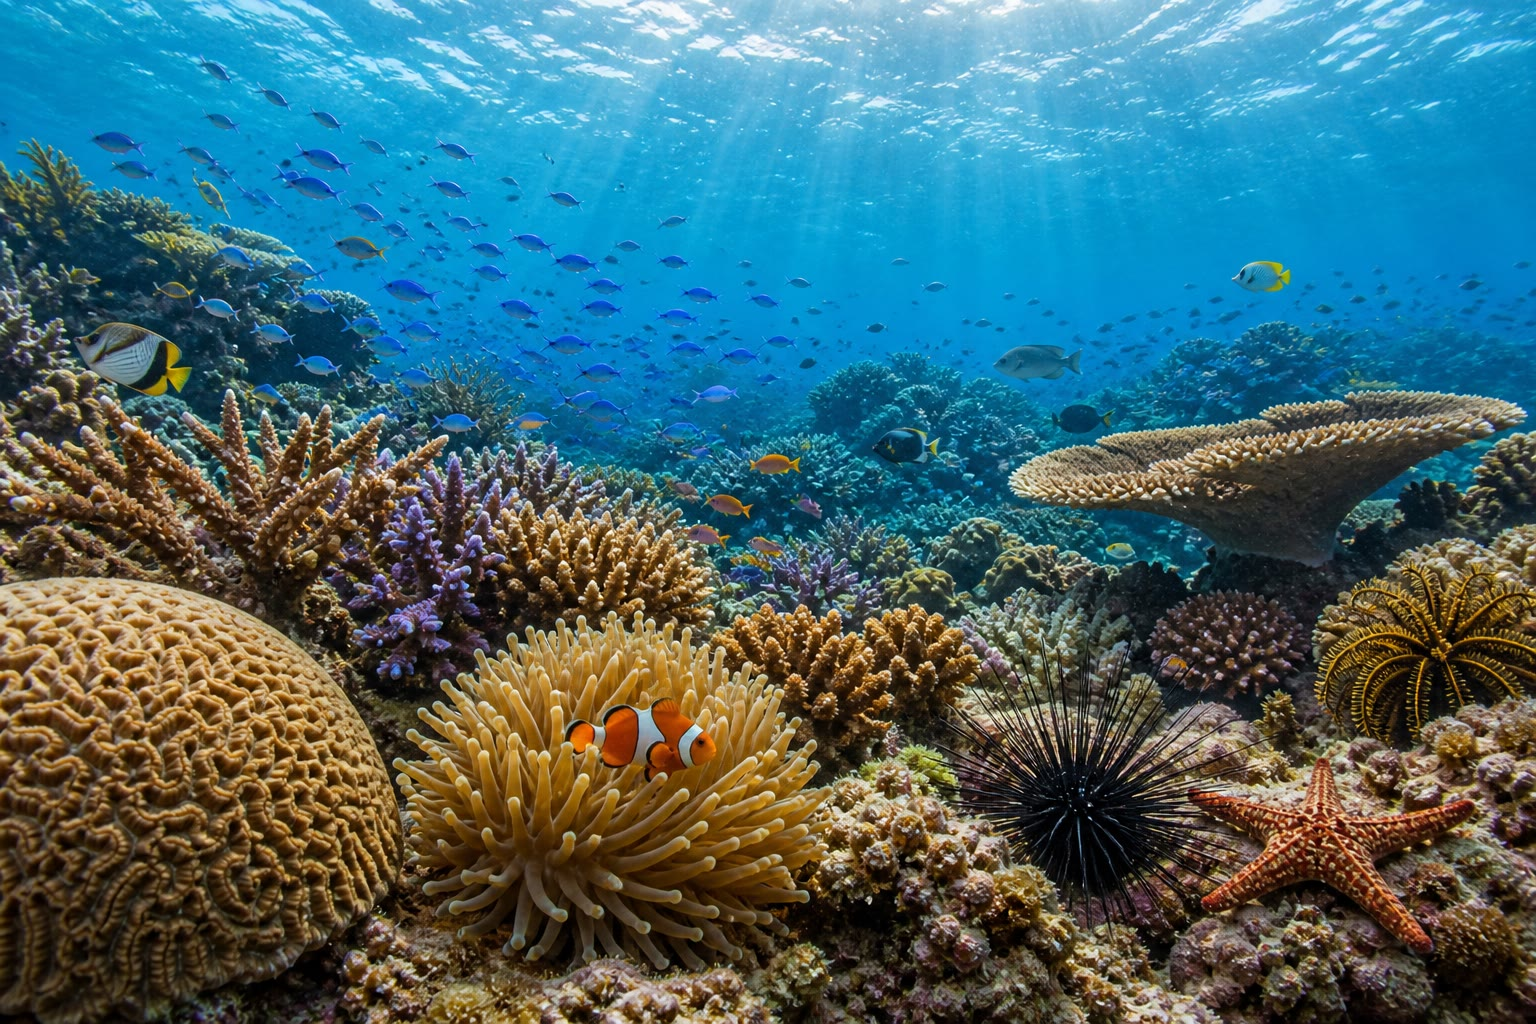
\includegraphics[width=0.66\linewidth]{images/book2/ai/g10-biodiv-coral-reef.jpg}

{\small Um recife de corais: em poucos metros quadrados, corais,
peixes, moluscos, equinodermos e anêmonas de dezenas de \omterm{def:g10:biodiversity-scales:species}{espécies}. Os
recifes abrigam um quarto de todas as \omterm{def:g10:biodiversity-scales:species}{espécies} marinhas em um décimo de
por cento do fundo do oceano.}
\end{omfigure}

\section{A diversidade genética dentro de uma espécie}

\begin{proposition}[Os indivíduos de uma espécie não são idênticos]\label{prop:g10:biodiversity-scales:genetic}
Dentro de uma \omterm{def:g10:biodiversity-scales:species}{espécie}, a maioria dos \omterm{def:g10:universal-dna:gene}{genes} existe em vários \omterm{def:g10:universal-dna:gene}{alelos}, e
os indivíduos carregam combinações diferentes deles. A
\emph{frequência} de um \omterm{def:g10:universal-dna:gene}{alelo} numa população --- a fração de todas as
cópias do \omterm{def:g10:universal-dna:gene}{gene} que são esse \omterm{def:g10:universal-dna:gene}{alelo} --- varia de uma população para
outra. A \omterm{def:g10:biodiversity-scales:biodiversity}{diversidade genética} é o que permite a uma \omterm{def:g10:biodiversity-scales:species}{espécie} responder a
um ambiente que muda: uma população em que todo indivíduo é igual não
tem de onde selecionar.
\end{proposition}
\admitted

\begin{example}[Os alelos dos grupos sanguíneos pelo mundo]\label{ex:g10:biodiversity-scales:abo}
O \omterm{def:g10:universal-dna:gene}{gene} dos grupos sanguíneos ABO tem três \omterm{def:g10:universal-dna:gene}{alelos} comuns, A, B e O. Na
Europa ocidental as frequências deles são de cerca de 0.27, 0.07 e
0.66; no leste da Ásia, cerca de 0.20, 0.20 e 0.60; em algumas
populações originárias da América do Sul o \omterm{def:g10:universal-dna:gene}{alelo} O sozinho chega a
0.98. Mesma \omterm{def:g10:biodiversity-scales:species}{espécie}, mesmo \omterm{def:g10:universal-dna:gene}{gene}, distribuições diferentes dos \omterm{def:g10:universal-dna:gene}{alelos}
dele: a \omterm{def:g10:biodiversity-scales:biodiversity}{diversidade genética} dos seres humanos é real, e ela está
espalhada entre as populações em vez de separá-las --- a maior parte da
diversidade da \omterm{def:g10:biodiversity-scales:species}{espécie} se encontra dentro de qualquer população.
\end{example}

\begin{omfigure}
\begin{tikzpicture}
\begin{axis}[
  ybar, bar width=9pt,
  width=0.8\linewidth, height=5.2cm,
  axis x line=bottom, axis y line=left,
  ymin=0, ymax=1.1, ylabel={frequência do alelo}, ylabel style={font=\small},
  symbolic x coords={Europa ocidental, leste da Ásia, Andes},
  xtick=data, tick label style={font=\small},
  enlarge x limits=0.25,
  legend style={at={(0.5,-0.2)}, anchor=north, legend columns=3,
                font=\small, draw=none},
  ytick={0,0.2,0.4,0.6,0.8,1.0},
]
\addplot[fill=omThm!50, draw=omThm] coordinates {(Europa ocidental,0.27) (leste da Ásia,0.20) (Andes,0.01)};
\addplot[fill=omProp!50, draw=omProp] coordinates {(Europa ocidental,0.07) (leste da Ásia,0.20) (Andes,0.01)};
\addplot[fill=omDef!50, draw=omDef] coordinates {(Europa ocidental,0.66) (leste da Ásia,0.60) (Andes,0.98)};
\legend{alelo A, alelo B, alelo O}
\end{axis}
\end{tikzpicture}

{\small Frequências aproximadas dos três \omterm{def:g10:universal-dna:gene}{alelos} ABO em três populações
humanas. As três frequências de uma população somam 1.}
\end{omfigure}

\begin{example}[Uma espécie quase sem nenhuma]\label{ex:g10:biodiversity-scales:cheetah}
Os guepardos são tão parecidos geneticamente que enxertos de pele entre
animais sem parentesco são aceitos como se fossem entre gêmeos: a
\omterm{def:g10:biodiversity-scales:species}{espécie} passou por um gargalo de pouquíssimos indivíduos há uns dez mil
anos e nunca recuperou os \omterm{def:g10:universal-dna:gene}{alelos} dela. Venha qual doença ou clima novo
vier, todo guepardo o enfrenta com o mesmo equipamento; a \omterm{def:g10:biodiversity-scales:species}{espécie}
sobrevive, mas sem nada de reserva.
\end{example}

\section{A biodiversidade muda: passado, presente}

\begin{proposition}[A biodiversidade é um estado, não uma constante]\label{prop:g10:biodiversity-scales:changes}
O conjunto de \omterm{def:g10:biodiversity-scales:species}{espécies} vivas num dado momento é uma etapa de uma
história. O registro fóssil mostra \omterm{def:g10:biodiversity-scales:species}{espécies} aparecendo, persistindo por
alguns milhões de anos em média e desaparecendo; a diversidade total da
vida aumentou ao longo dos últimos 540 milhões de anos, interrompida
por cinco \emph{extinções em massa}\index{extinção em massa} em que
mais de três quartos das \omterm{def:g10:biodiversity-scales:species}{espécies} sumiram num intervalo geologicamente
curto. A mais recente, há 66 milhões de anos, acabou com os dinossauros
não aviários e abriu caminho para a diversificação dos mamíferos.
\end{proposition}
\begin{proof}[Evidências]
Contagens de famílias fósseis em camadas de rocha datadas, compiladas
para todo o registro marinho, dão a curva da figura seguinte: uma
subida de algumas centenas a quase mil famílias, com quedas bruscas há
445, 370, 252, 201 e 66 milhões de anos. O evento de 252 milhões de
anos, o maior, eliminou cerca de 95\% das \omterm{def:g10:biodiversity-scales:species}{espécies} marinhas; as camadas
logo acima dele estão quase vazias de fósseis, e novos grupos só as
preenchem ao longo dos milhões de anos seguintes.
\end{proof}

\begin{omfigure}
\begin{tikzpicture}
\begin{axis}[
  width=0.9\linewidth, height=5.6cm,
  axis x line=bottom, axis y line=left,
  x dir=reverse, xmin=0, xmax=560, ymin=0, ymax=1100,
  xlabel={milhões de anos atrás}, ylabel={famílias de animais marinhos},
  xlabel style={font=\small, at={(axis description cs:0.5,-0.12)}, anchor=north},
  ylabel style={font=\small},
  tick label style={font=\small}, xtick={500,400,300,200,100,0},
  ytick={0,200,400,600,800,1000},
  clip=false,
]
\addplot[thick, omDef] coordinates
  {(540,120) (520,300) (490,420) (460,500) (447,510) (440,400)
   (420,470) (380,530) (368,540) (360,450) (330,480) (300,520)
   (260,540) (252,560) (248,300) (230,380) (210,440) (202,450)
   (196,380) (150,520) (100,650) (70,760) (66,780) (62,650)
   (40,760) (20,880) (0,1000)};
\draw[thick, omThm, ->] (axis cs:445,760) -- (axis cs:445,600);
\node[font=\scriptsize, omThm, anchor=south] at (axis cs:445,770) {1};
\draw[thick, omThm, ->] (axis cs:370,790) -- (axis cs:370,630);
\node[font=\scriptsize, omThm, anchor=south] at (axis cs:370,800) {2};
\draw[thick, omThm, ->] (axis cs:252,820) -- (axis cs:252,660);
\node[font=\scriptsize, omThm, anchor=south] at (axis cs:252,830) {3};
\draw[thick, omThm, ->] (axis cs:201,700) -- (axis cs:201,540);
\node[font=\scriptsize, omThm, anchor=south] at (axis cs:201,710) {4};
\draw[thick, omThm, ->] (axis cs:66,1030) -- (axis cs:66,870);
\node[font=\scriptsize, omThm, anchor=south] at (axis cs:66,1040) {5};
\end{axis}
\end{tikzpicture}

{\small Número de famílias de animais marinhos ao longo do tempo, a
partir do registro fóssil, com as cinco \omterm{prop:g10:biodiversity-scales:changes}{extinções em massa} marcadas
(1: fim do Ordoviciano; 2: Devoniano tardio; 3: fim do Permiano, a
maior; 4: fim do Triássico; 5: fim do Cretáceo). A diversidade sobe no
conjunto, e cada colapso é seguido de uma recuperação lenta.}
\end{omfigure}

\begin{proposition}[A mudança em curso]\label{prop:g10:biodiversity-scales:present}
As \omterm{def:g10:biodiversity-scales:species}{espécies} estão desaparecendo hoje a uma taxa estimada em cem a mil
vezes a média do registro fóssil, por causa da destruição de
\omterm{def:g10:biodiversity-scales:biodiversity}{ecossistemas} (desmatamento, drenagem de áreas úmidas, urbanização), da
superexploração, de \omterm{def:g10:biodiversity-scales:species}{espécies} introduzidas, da poluição e da mudança do
clima --- tudo de origem humana. Metade das florestas tropicais de 1950
já se foi; um terço das \omterm{def:g10:biodiversity-scales:species}{espécies} de anfíbios está ameaçado; a
\omterm{def:g10:biodiversity-scales:biodiversity}{diversidade genética} das lavouras e dos rebanhos se estreitou a umas
poucas variedades. A \omterm{def:g10:biodiversity-scales:biodiversity}{biodiversidade} é um recurso --- alimento,
medicamentos, polinização, solo, estabilidade dos \omterm{def:g10:biodiversity-scales:biodiversity}{ecossistemas} --- e a
perda dela não é reversível numa escala de tempo humana.
\end{proposition}
\admitted

\begin{example}[Reverter uma perda]\label{ex:g10:biodiversity-scales:reversing}
Onde cercas vivas arrancadas nos anos 1960 foram replantadas, a riqueza
de aves e de insetos volta em uma década; onde os lobos foram
reintroduzidos num parque nacional em 1995, os cervos que eles caçam
pararam de descascar os salgueiros da beira do rio, os salgueiros
rebrotaram, os castores voltaram, e com eles as aves e os peixes que
dependem dos açudes de castor. Proteger ou restaurar um \omterm{def:g10:biodiversity-scales:biodiversity}{ecossistema}
restaura a diversidade nas três escalas ao mesmo tempo; uma \omterm{def:g10:biodiversity-scales:species}{espécie}
mantida viva num zoológico conserva apenas uma delas.
\end{example}

\section{Exercícios}

\begin{exercise}[$\star$]\label{exo:g10:biodiversity-scales:1}
Cite as três escalas da \omterm{def:g10:biodiversity-scales:biodiversity}{biodiversidade} e dê um exemplo de cada uma.
\end{exercise}

\begin{exercise}[$\star$]\label{exo:g10:biodiversity-scales:2}
Defina \omterm{def:g10:biodiversity-scales:species}{espécie}. O leão e o tigre --- que conseguem produzir híbridos
estéreis em cativeiro --- são uma \omterm{def:g10:biodiversity-scales:species}{espécie} ou duas?
\end{exercise}

\begin{exercise}[$\star$]\label{exo:g10:biodiversity-scales:3}
A partir do gráfico das \omterm{def:g10:biodiversity-scales:species}{espécies}, quantas vezes mais \omterm{def:g10:biodiversity-scales:species}{espécies} de
insetos que de mamíferos já foram descritas?
\end{exercise}

\begin{exercise}[$\star$]\label{exo:g10:biodiversity-scales:4}
O que é a frequência de um \omterm{def:g10:universal-dna:gene}{alelo}? Numa população em que o \omterm{def:g10:universal-dna:gene}{alelo} O tem
frequência 0.66 e o \omterm{def:g10:universal-dna:gene}{alelo} A, 0.27, qual é a frequência de B?
\end{exercise}

\begin{exercise}[$\star$]\label{exo:g10:biodiversity-scales:5}
Quantas \omterm{prop:g10:biodiversity-scales:changes}{extinções em massa} o registro fóssil mostra, e qual foi a maior?
\end{exercise}

\begin{exercise}[$\star\star$]\label{exo:g10:biodiversity-scales:6}
Dois prados têm 12 \omterm{def:g10:biodiversity-scales:species}{espécies} de plantas cada um. No primeiro, uma
\omterm{def:g10:biodiversity-scales:species}{espécie} faz 80\% das plantas; no segundo, nenhuma \omterm{def:g10:biodiversity-scales:species}{espécie} passa de
15\%. Qual é mais diverso, e qual dos dois números do
\cref{met:g10:biodiversity-scales:sampling} os distingue?
\end{exercise}

\begin{exercise}[$\star\star$]\label{exo:g10:biodiversity-scales:7}
Um aluno conta insetos em 3 passadas de rede e encontra 8 \omterm{def:g10:biodiversity-scales:species}{espécies}; uma
colega faz 30 passadas no mesmo campo e encontra 21. O campo tem mais
\omterm{def:g10:biodiversity-scales:species}{espécies} para a colega? Explique o que a diferença mostra sobre a
amostragem.
\end{exercise}

\begin{exercise}[$\star\star$]\label{exo:g10:biodiversity-scales:8}
Explique por que uma \omterm{def:g10:biodiversity-scales:species}{espécie} reduzida a algumas dezenas de indivíduos
pode continuar em perigo mesmo depois de os números dela voltarem aos
milhares.
\end{exercise}

\begin{exercise}[$\star\star$]\label{exo:g10:biodiversity-scales:9}
Na figura das famílias fósseis, leia o número de famílias logo antes e
logo depois da extinção de 252 milhões de anos atrás, e calcule a
fração perdida. Por que a fração de \emph{\omterm{def:g10:biodiversity-scales:species}{espécies}} perdidas é maior
que a fração de famílias?
\end{exercise}

\begin{exercise}[$\star\star$]\label{exo:g10:biodiversity-scales:10}
Usando o \cref{ex:g10:biodiversity-scales:abo}, explique em que sentido
dois vizinhos de uma mesma cidade provavelmente diferem geneticamente
mais ou menos tanto quanto duas pessoas de continentes diferentes.
\end{exercise}

\begin{exercise}[$\star\star$]\label{exo:g10:biodiversity-scales:11}
Uma lagoa é drenada para construir um estacionamento. Liste uma perda
em cada uma das três escalas da \omterm{def:g10:biodiversity-scales:biodiversity}{biodiversidade}.
\end{exercise}

\begin{exercise}[$\star\star\star$]\label{exo:g10:biodiversity-scales:12}
A \omterm{def:g10:biodiversity-scales:species}{espécie} média do registro fóssil dura alguns milhões de anos; com
dois milhões de \omterm{def:g10:biodiversity-scales:species}{espécies} conhecidas, estime o número ``de fundo'' de
extinções por ano. Se a taxa atual é mil vezes maior, quantas \omterm{def:g10:biodiversity-scales:species}{espécies}
desapareceriam por ano, e quantas por século?
\end{exercise}

\begin{exercise}[$\star\star\star$]\label{exo:g10:biodiversity-scales:13}
Depois da extinção de 66 milhões de anos atrás, os mamíferos se
diversificaram de algumas poucas formas pequenas em baleias, morcegos,
elefantes e primatas em uns 20 milhões de anos. Explique como uma
catástrofe para a \omterm{def:g10:biodiversity-scales:biodiversity}{biodiversidade} pode ser também uma causa de nova
\omterm{def:g10:biodiversity-scales:biodiversity}{biodiversidade}.
\end{exercise}

\begin{exercise}[$\star\star\star$]\label{exo:g10:biodiversity-scales:14}
O trigo moderno descende de um punhado de variedades; os parentes
silvestres dele crescem nas montanhas do Oriente Médio. Explique, com a
noção de \omterm{def:g10:biodiversity-scales:biodiversity}{diversidade genética}, por que os bancos de sementes conservam
os parentes silvestres mesmo que eles não rendam nada aproveitável.
\end{exercise}

\begin{exercise}[$\star\star\star$]\label{exo:g10:biodiversity-scales:15}
``A extinção é natural, logo não há razão para se preocupar com a
atual.'' Discuta num parágrafo usando a taxa de extinção, o tempo de
recuperação e os recursos que a \omterm{def:g10:biodiversity-scales:biodiversity}{biodiversidade} fornece.
\end{exercise}

\section{Problema: o dividendo da cerca viva}

\begin{problem}[{Problema de fim de semana --- um levantamento de campo
em duas fazendas, uma com cercas vivas e outra sem: espécies contadas,
abundâncias comparadas, os alelos de um caracol acompanhados, e quanto
vale uma cerca viva}]
\label{pb:g10:biodiversity-scales:1}
Duas fazendas vizinhas cultivam o mesmo trigo no mesmo solo. A fazenda
A manteve as cercas vivas dela; a fazenda B arrancou as dela em 1970.
Uma turma faz amostragem nas duas em junho com o mesmo método: 20
parcelas de \qty{1}{m^2} ao longo das bordas dos campos para as
plantas, 20 passadas de rede para os insetos e 10 minutos de escuta em
5 pontos para as aves.

\medskip
\noindent\textbf{Parte I --- As plantas.}
Resultados, fazenda A: 31 \omterm{def:g10:biodiversity-scales:species}{espécies} de plantas nas 20 parcelas; fazenda
B: 9. Na fazenda B, uma gramínea faz 84\% das plantas contadas; na
fazenda A a \omterm{def:g10:biodiversity-scales:species}{espécie} mais comum faz 22\%.
\begin{enumerate}
  \item Dê a riqueza de \omterm{def:g10:biodiversity-scales:species}{espécies} das bordas de cada fazenda e a razão
        entre elas.
  \item A comunidade vegetal de qual fazenda é mais uniforme? Explique
        o que ``uniforme'' acrescenta a ``rica''.
  \item Na fazenda A, o número de \omterm{def:g10:biodiversity-scales:species}{espécies} encontradas depois de 5, 10,
        15 e 20 parcelas foi 18, 25, 29 e 31. A amostragem é
        suficiente? Justifique.
  \item A mesma série na fazenda B foi 6, 8, 9, 9. Compare as duas
        séries e diga que forma toma uma curva de amostragem
        ``completa''.
  \item Por que as duas fazendas precisam ser amostradas no mesmo mês?
\end{enumerate}

\medskip
\noindent\textbf{Parte II --- Insetos e aves.}
Insetos: fazenda A 46 \omterm{def:g10:biodiversity-scales:species}{espécies}, fazenda B 14. Aves: fazenda A 17
\omterm{def:g10:biodiversity-scales:species}{espécies}, fazenda B 5; na fazenda B, 60\% das aves ouvidas eram de uma
única \omterm{def:g10:biodiversity-scales:species}{espécie}.
\begin{enumerate}[resume]
  \item Calcule a razão da riqueza de insetos e a da riqueza de aves
        entre as fazendas. Os três grupos (plantas, insetos, aves)
        contam a mesma história?
  \item Proponha uma cadeia de causas ligando a retirada das cercas
        vivas à queda da diversidade de insetos, e depois à das aves.
  \item A produtividade de trigo por hectare é a mesma nas duas
        fazendas. Isso quer dizer que as cercas vivas não têm efeito
        sobre a lavoura? Sugira um serviço que uma cerca viva pode
        prestar e que o número da produtividade não mostra.
  \item Cite uma \omterm{def:g10:biodiversity-scales:species}{espécie} que a turma esperaria encontrar somente na
        fazenda A e explique por quê.
  \item Que escala da \omterm{def:g10:biodiversity-scales:biodiversity}{biodiversidade} foi mais claramente reduzida na
        fazenda B: os \omterm{def:g10:biodiversity-scales:biodiversity}{ecossistemas}, as \omterm{def:g10:biodiversity-scales:species}{espécies} ou os \omterm{def:g10:universal-dna:gene}{genes}? Justifique.
\end{enumerate}

\medskip
\noindent\textbf{Parte III --- Os \omterm{def:g10:universal-dna:gene}{alelos} de um caracol.}
O caracol-dos-bosques carrega um \omterm{def:g10:universal-dna:gene}{gene} com dois \omterm{def:g10:universal-dna:gene}{alelos} comuns para a cor
da concha, amarelo (y) e marrom (b). Nas cercas vivas da fazenda A,
foram amostrados 400 caracóis: 100 têm dois \omterm{def:g10:universal-dna:gene}{alelos} y, 200 têm um y e um
b, 100 têm dois b. No único barranco que resta na fazenda B, 100
caracóis: 4 com dois y, 32 com um de cada, 64 com dois b.
\begin{enumerate}[resume]
  \item Conte as cópias de y e de b em cada amostra (cada caracol
        carrega duas cópias). Deduza a frequência de y em cada fazenda.
  \item Qual população é geneticamente mais diversa nesse \omterm{def:g10:universal-dna:gene}{gene}?
        Compare a proporção de caracóis que carregam os dois \omterm{def:g10:universal-dna:gene}{alelos}.
  \item Os sabiás caçam caracóis pela visão; no barranco descoberto da
        fazenda B, as conchas marrons ficam mais escondidas. Proponha
        como surgiram as frequências da fazenda B.
  \item Se uma cerca viva úmida e sombreada favorecesse as conchas
        amarelas, o que você preveria para os caracóis da fazenda B se
        as cercas fossem replantadas e nada mais mudasse?
  \item Os caracóis da fazenda B somam algumas centenas; os da fazenda
        A, dezenas de milhares. Que população está mais exposta a
        perder um \omterm{def:g10:universal-dna:gene}{alelo} por completo por acaso? Por quê?
\end{enumerate}

\medskip
\noindent\textbf{Parte IV --- O dividendo.}
\begin{enumerate}[resume]
  \item Somando os três grupos, calcule a riqueza total de \omterm{def:g10:biodiversity-scales:species}{espécies} de
        cada fazenda, depois o total da fazenda A dividido pelo da
        fazenda B.
  \item As cercas vivas da fazenda A ocupam 3\% da área dela. Enuncie
        numa frase que fração da terra está abrigando que fração das
        \omterm{def:g10:biodiversity-scales:species}{espécies}.
  \item As cercas vivas replantadas na fazenda B em 1995 foram
        recenseadas de novo em 2010: 24 \omterm{def:g10:biodiversity-scales:species}{espécies} de plantas, 35 de
        insetos, 12 de aves. Que fração da riqueza da fazenda A cada
        grupo tinha recuperado?
  \item Qual das três escalas da \omterm{def:g10:biodiversity-scales:biodiversity}{biodiversidade} se recupera mais devagar
        depois do replantio, e por quê?
  \item Enuncie o resultado: o fator pelo qual as cercas vivas
        multiplicaram a riqueza de \omterm{def:g10:biodiversity-scales:species}{espécies} de uma fazenda, e a única
        escala da \omterm{def:g10:biodiversity-scales:biodiversity}{biodiversidade} que uma cerca viva replantada não
        consegue trazer de volta sozinha.
\end{enumerate}
\end{problem}
